\appendix
\chapter{The Appendix}
This appendix lists mainly figures that highlight interesting or surprising behaviours but only serve to support the want for a more detailed picture and are not relevant for the main points. 

The code for the simulations in this report were written using Julia\cite{Julia-2017} and would not have been possible without its extensive standard library and package ecosystem, including but not limited to \texttt{Graphs.jl}\cite{Graphs2021} for the network side and \texttt{Makie.jl}\cite{DanischKrumbiegel2021} for visualization.

\chapter[Task 01]{\#01 Ising Model}
As seen in figure \ref{fig:cv-chi-01} the curves of susceptibility and heat capacity do not peak for the same temperature and are relatively noisy with large variations.
\begin{figure}[h]
	\centering
	\includegraphics[width=0.5\textwidth]{Ising\_CvChi\_SF\_32}
	\caption{Behaviour of the susceptibility and heat capacity for a scale free network with a degree exponent of 3.2}
	\label{fig:cv-chi-01}
\end{figure}

\begin{figure}[h!]
	\centering
	\includegraphics[width=0.6\textwidth]{Ising\_EM\_SF\_20}
	\caption{Behaviour of the energy and magnetization for a scale free network with a degree exponent of 2}
	\label{fig:EM-SF-2.0-01}
\end{figure}
In figure \ref{fig:EM-SF-2.0-01} I show that M and E do not stay near 1, which would be indicative of the always ferromagnetic behaviour, as it is described in \cite{Leone2002} to happen. It is remarkable though that the transition seems to begin for rather low temperatures and then continue very slowly.

In figure \ref{fig:SF-comp-theory-01} a variety of target thresholds is compared to determine the critical
\begin{figure}[h]
	\centering
	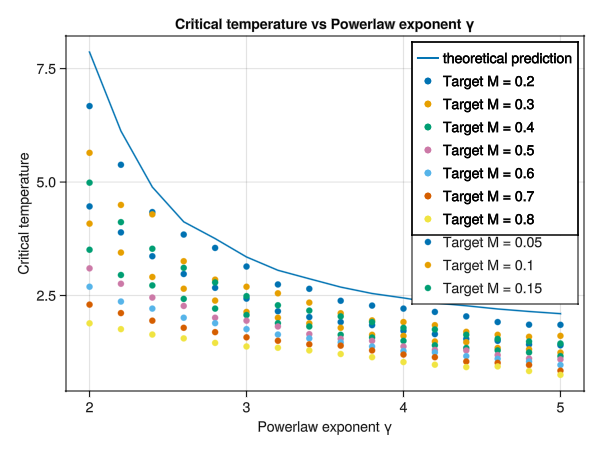
\includegraphics{phase_diagram_cutoff_variable_powerlaw}
	\caption{Behaviour of the critical temperature as determined by various thresholds}
	\label{fig:SF-comp-theory-01}
\end{figure}
temperature from. It is visible that for a threshold too large the temperature is much too low while a very small one leads to very noisy estimate. The optimal one seems to be at \numrange{0.03}{0.05}.

\chapter[Task 16]{\#16: Traffic Congestion}

\begin{figure}[h]
	\centering
	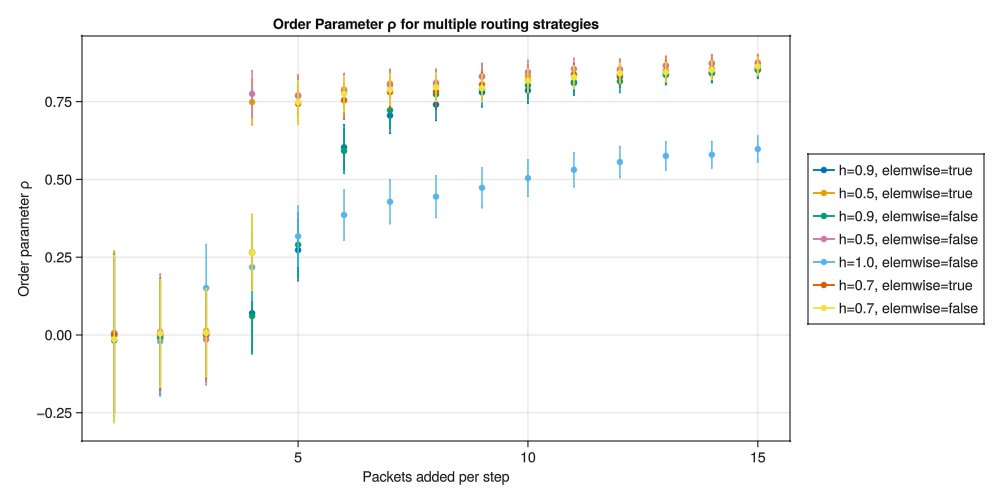
\includegraphics{reduced_plot_h_elemwise_pps}
	\caption{Comparison of different path length modifiers and neighbour choice algorithms. Application of the effective distance function for each step of the way.}
	\label{fig:elemwise-allscaled-16}
\end{figure}


\chapter[Task 41]{\#41 Public Transport in Large Cities Worldwide}
\begin{figure}[h]
	\centering
	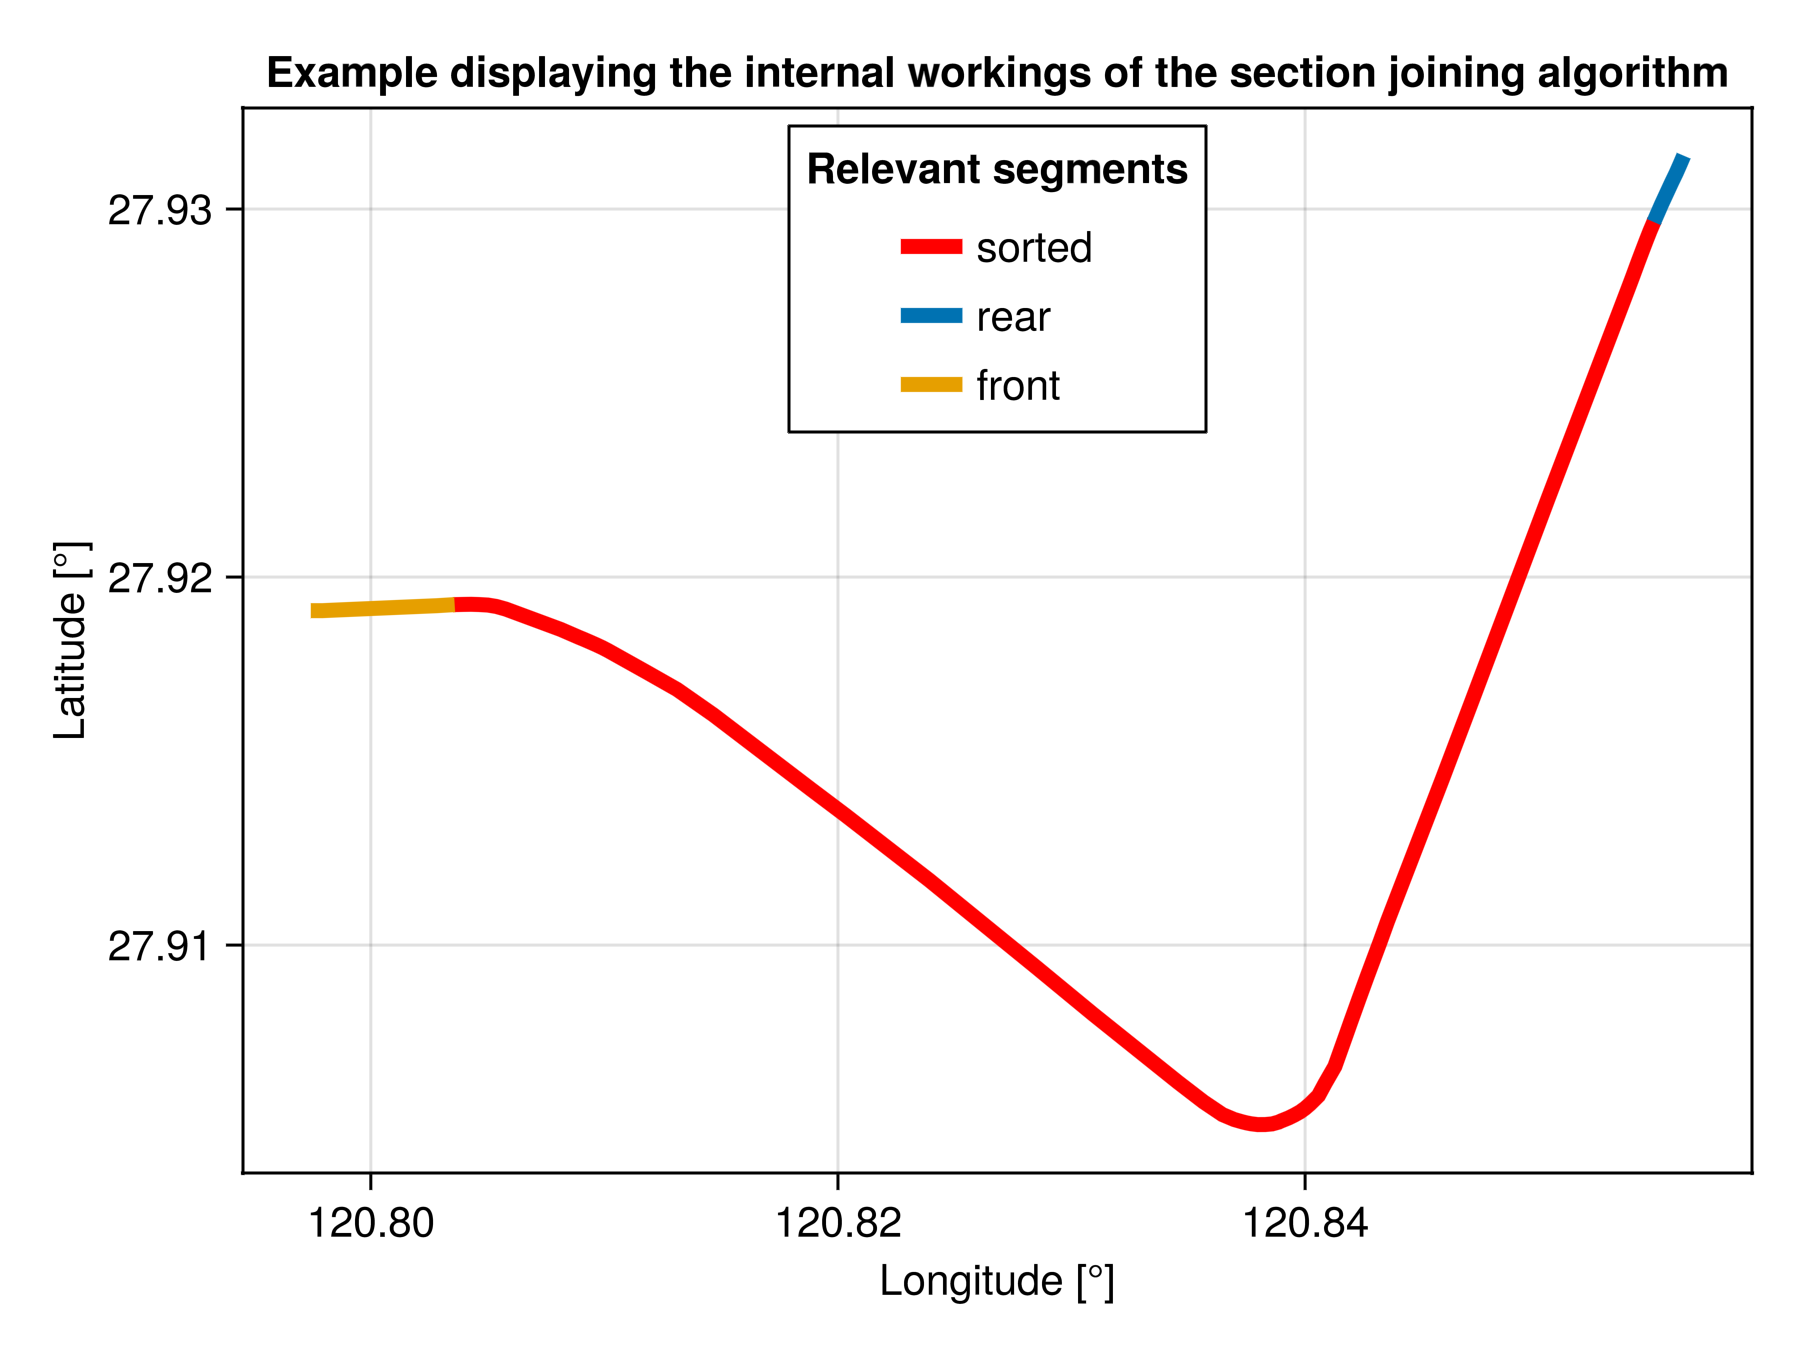
\includegraphics[width=0.4\textwidth]{algorithm_example_wenzhou}
	\caption{\centering This figure shows a snapshot of the algorithm described in section \ref{sec:algorithm-41}. `sorted' in the legend refers to the already joined segments, `rear' and `front' to the tail and head end of `sorted' respectively}
	\label{fig:algorithm-41}
\end{figure}

\begin{figure}[h]
	\centering
	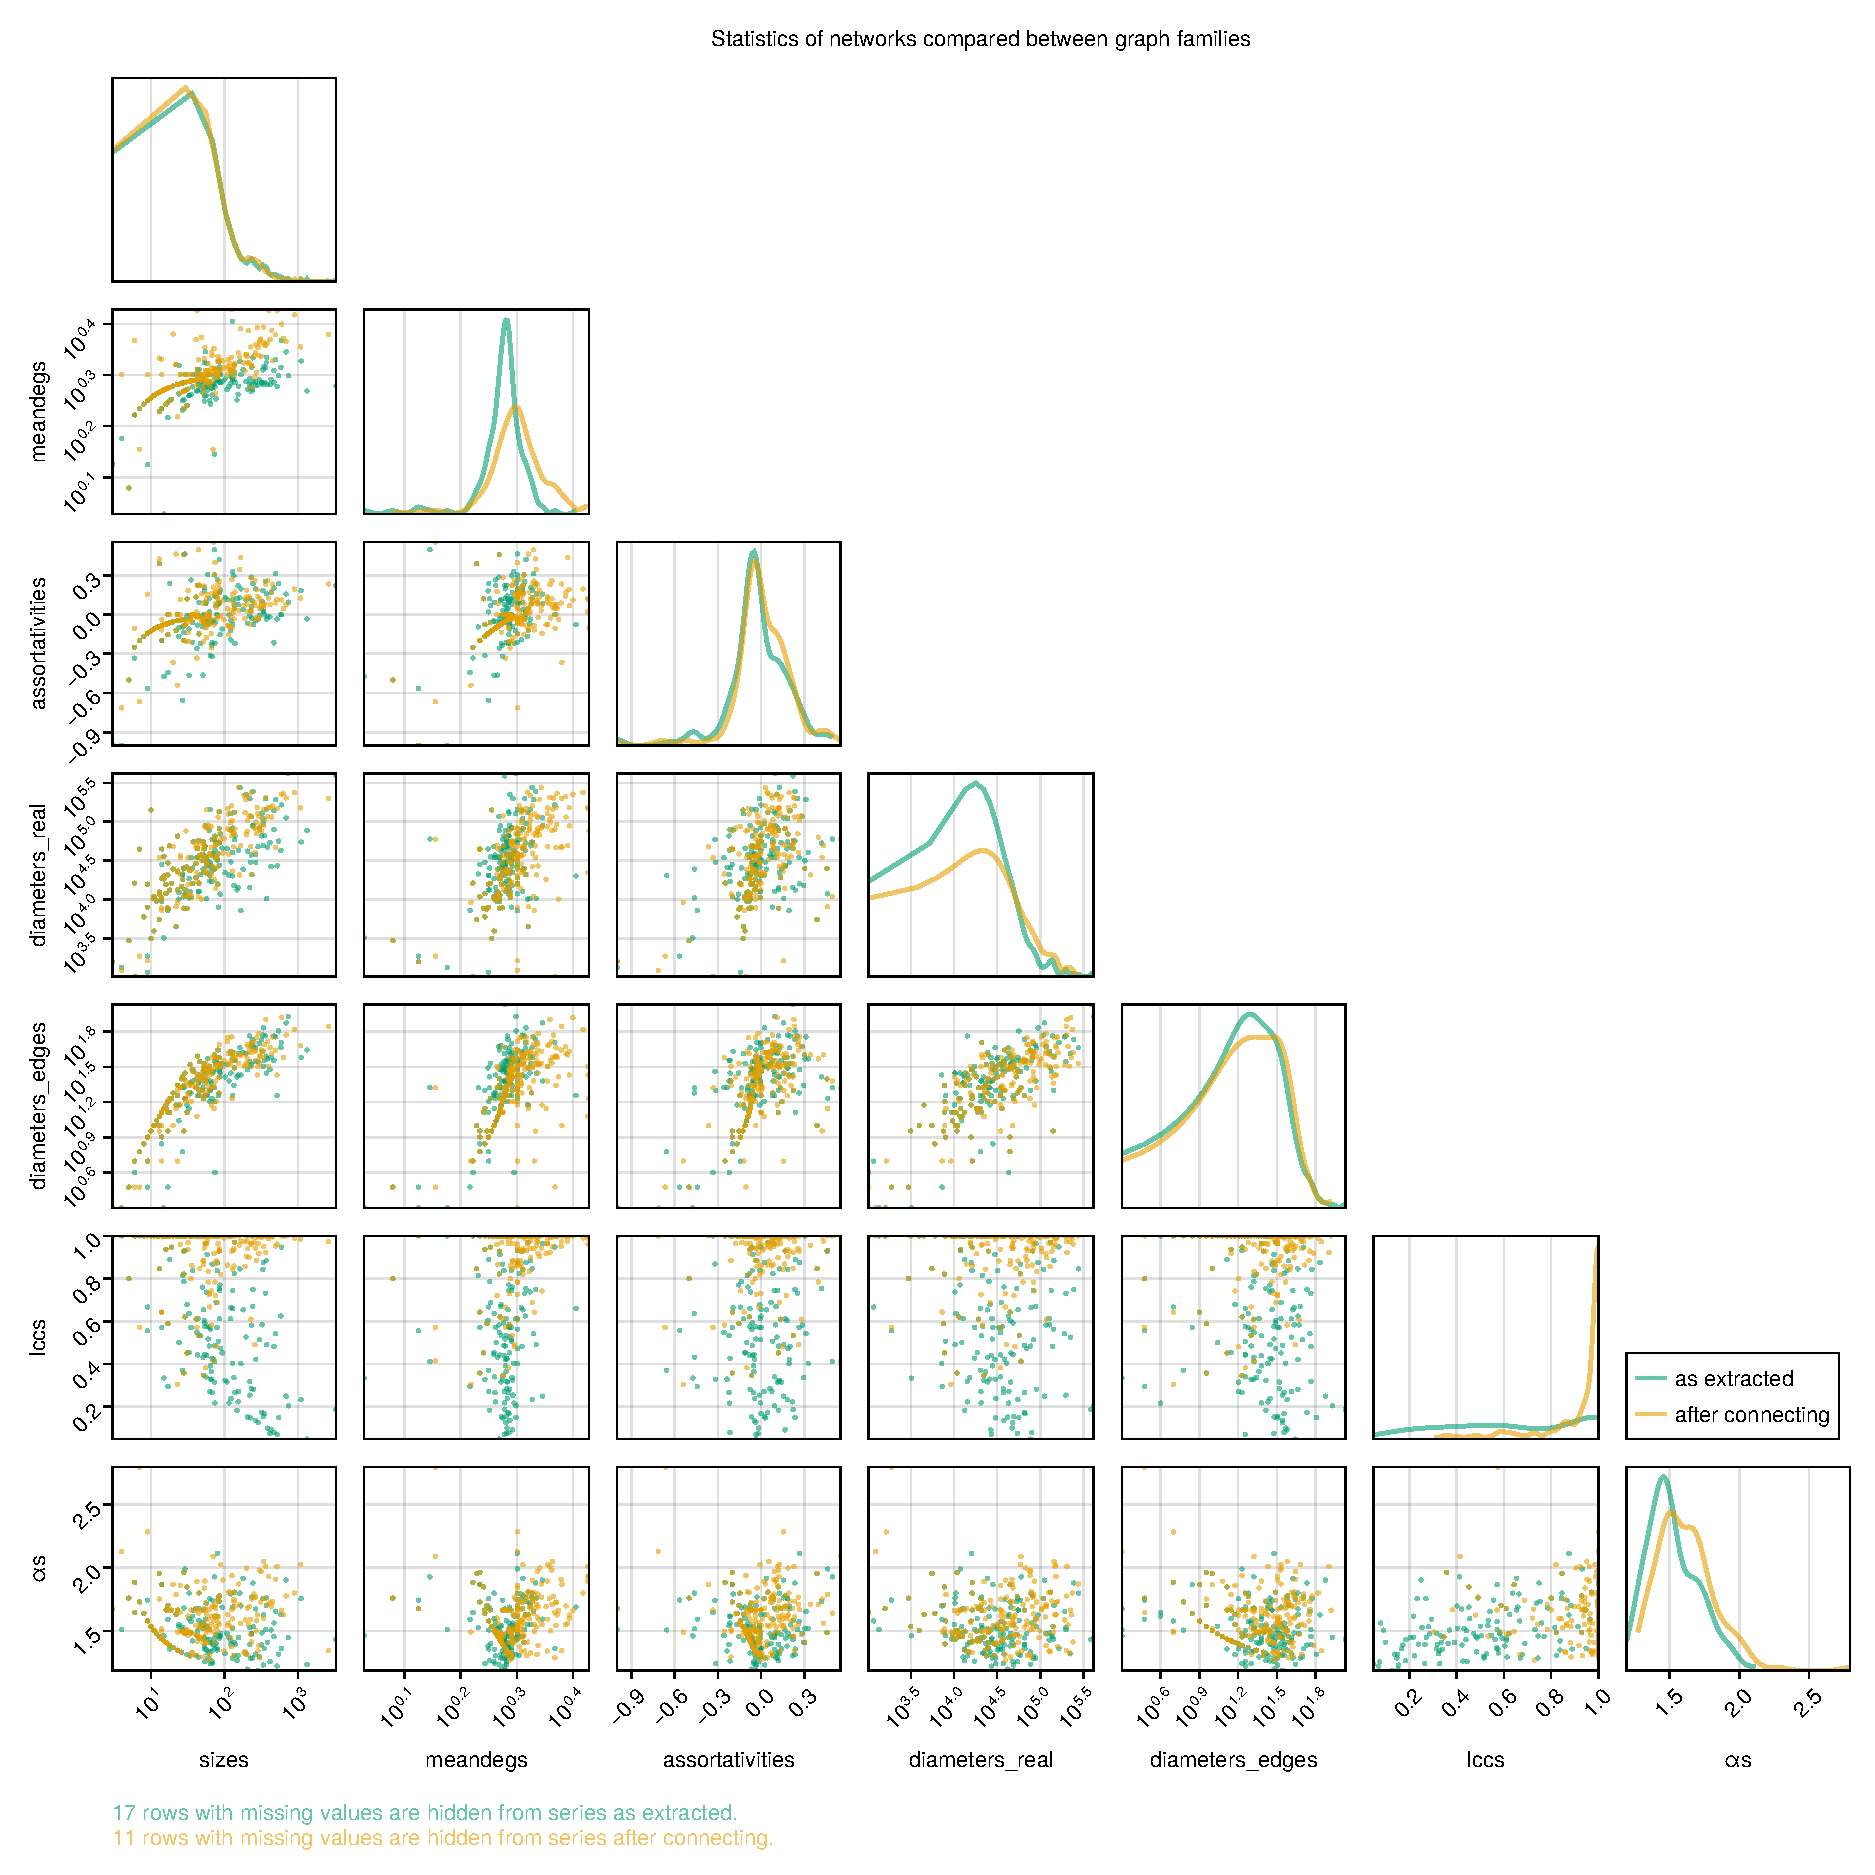
\includegraphics[width=\textwidth]{pairplot_both}
	\caption{Pairwise comparisons of the main graph metrics as named in section \ref{sec:analysis-41}}
	\label{fig:pairplots}
\end{figure}

\begin{table}[h]
	\centering
	\begin{tabular}{lrrrrr}
		\hline
		\textbf{variable} & \textbf{mean} & \textbf{min} & \textbf{median} & \textbf{max} & \textbf{nmissing}  \\\hline
		size & 139.0 & 3.0 & 57.0 & 3272.0 & 0 \\
		mean degree & 1.895 & 1.07 & 1.91 & 2.54 & 0  \\
		assortativity & -0.0335 & -1.0 & -0.0371 & 0.495 & 0 \\
		diameter [\unit{\meter}] & 46997.1 & 1028.13 & 27822.2 & 4.17e5 & 0  \\
		diameters [\#edges] & 26.6 & 2.0 & 24.0 & 107.0 & 0  \\
		relative size LCC & 0.646 & 0.0476 & 0.636 & 1.0 & 0  \\
		$\alpha$s & 1.521 & 1.192 & 1.486 & 2.12 & 18  \\\hline
	\end{tabular}
	\caption{Metric distribution in the graphs as extracted from the data}
\end{table}

\begin{table}[h]
	\centering
	\begin{tabular}{lrrrrr}
		\hline
		\textbf{variable} & \textbf{mean} & \textbf{min} & \textbf{median} & \textbf{max} & \textbf{nmissing} \\\hline
		size & 122.8 & 3.0 & 54.0 & 2608.0 & 0 \\
		mean degree & 2.024 & 1.2 & 2.0 & 2.683 & 0 \\
		assortativities & 0.00566591 & -1.0 & -0.00813008 & 0.552941 & 0 \\
		diameter [m] & 57132.6 & 1028.13 & 37181.1 & 2.75689e5 & 0 \\
		diameter [\#edges] & 27.1854 & 2.0 & 26.0 & 83.0 & 0 \\
		relative size LCC & 0.914744 & 0.304348 & 1.0 & 1.0 & 0 \\
		$\alpha$ & 1.61813 & 1.2724 & 1.59582 & 2.79234 & 11 \\\hline
	\end{tabular}
	\caption{Data distribution in the graphs after a node joining pass}
\end{table}

\newpage